\section{Analyse des métriques}

\subsection{Analyse des métriques pour la DHT naïve}

Cette sous-section regroupe les mesures obtenues pour la deuxième génération, c'est-à-dire l'architecture non structurée inspirée de \textit{Gnutella}. L'objectif n'est pas seulement de présenter les courbes expérimentales, mais aussi de relier leur forme aux mécanismes introduits dans l'implémentation : \textit{flooding}, \textit{pong caching}, \textit{reverse path caching} et convergence progressive vers un maillage dense.

\subsubsection{Latence moyenne des requêtes en fonction de la charge}

\begin{wrapfigure}{r}{0.44\textwidth}
    \centering
    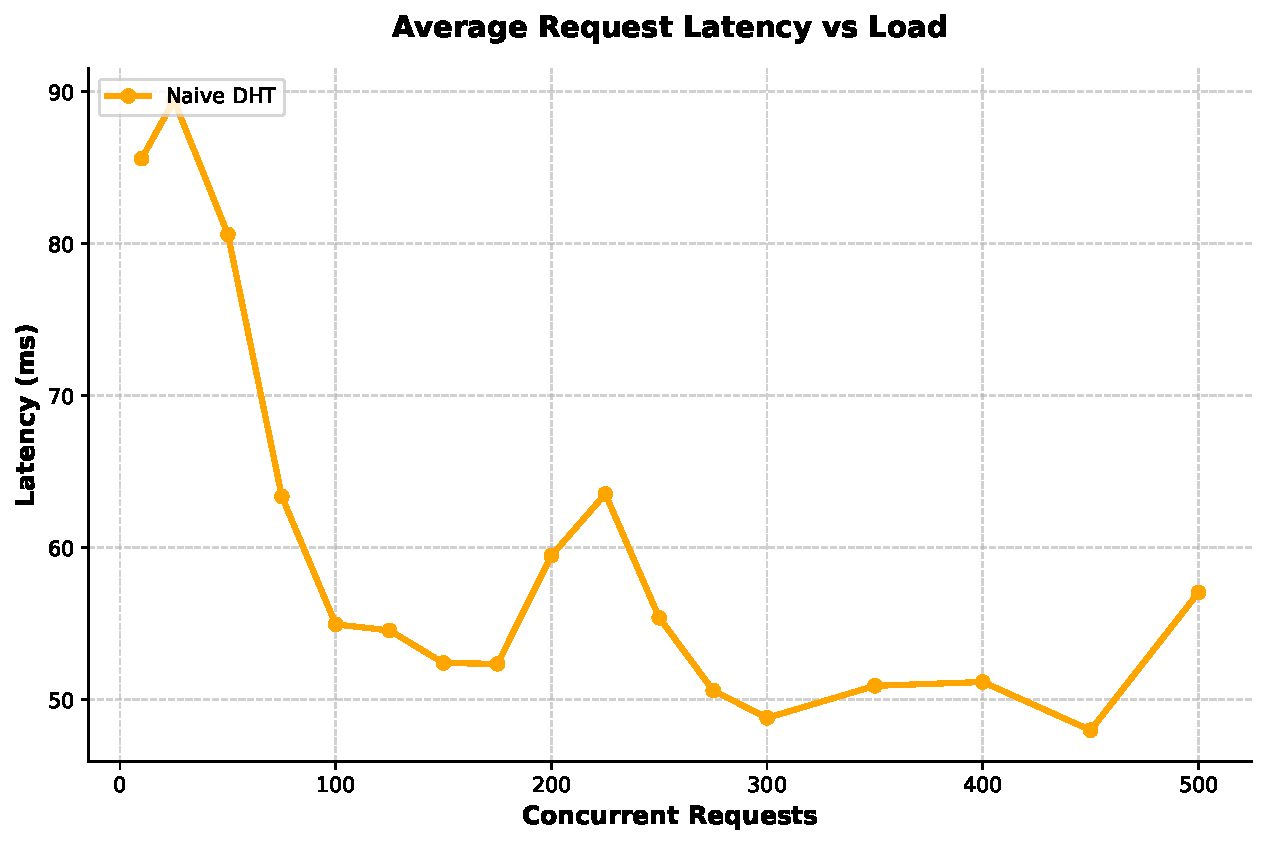
\includegraphics[width=0.40\textwidth]{graphs/pdf/dht_latency.pdf}
    \caption{Latence moyenne des requêtes en fonction de la charge dans la DHT naïve.}
    \label{fig:naive_metrics_latency}
\end{wrapfigure}

La Figure~\ref{fig:naive_metrics_latency} met en évidence un pic de latence initial, observé lorsque la charge est encore faible, puis une chute rapide vers une ligne de base beaucoup plus stable. Ce comportement est cohérent avec la présence du \textit{reverse path caching}. Lors des premières requêtes, la donnée n'est généralement pas encore présente à proximité du client ; la résolution dépend donc du coût complet du parcours réseau et d'un retour depuis le détenteur effectif de la donnée. Dans cette phase, la latence est essentiellement gouvernée par la distance parcourue dans le réseau et par le délai introduit à chaque saut.

Dans un tel régime, si l'on note \(D\) le diamètre effectif du réseau et \(L_{hop}\) le délai moyen associé à un saut, la latence d'une requête non mise en cache peut être majorée par un terme de l'ordre de
\[
L_{network} \in O(D \cdot L_{hop}).
\]
À mesure que les requêtes se répètent, le \textit{reverse path caching} diffuse des copies de la donnée sur les chemins les plus sollicités. Le taux de succès du cache, noté \(h\), augmente alors rapidement, ce qui permet de modéliser la latence moyenne globale par
\[
\bar{L} = h \cdot L_{cache} + (1-h) \cdot L_{network}.
\]
Lorsque la charge augmente, la redondance des accès rend plus probable la présence locale ou quasi locale de la donnée ; on tend ainsi vers \(h \to 1\), et la latence moyenne converge vers \(L_{cache}\), c'est-à-dire vers le coût d'un accès local, bien inférieur au coût d'un parcours réseau complet. La forme de la courbe valide donc empiriquement l'effet attendu de la mise en cache opportuniste : sous forte charge, le réseau est de moins en moins sollicité pour les données populaires.

\subsubsection{Débit global du système en fonction de la charge}

\begin{wrapfigure}{l}{0.44\textwidth}
    \centering
    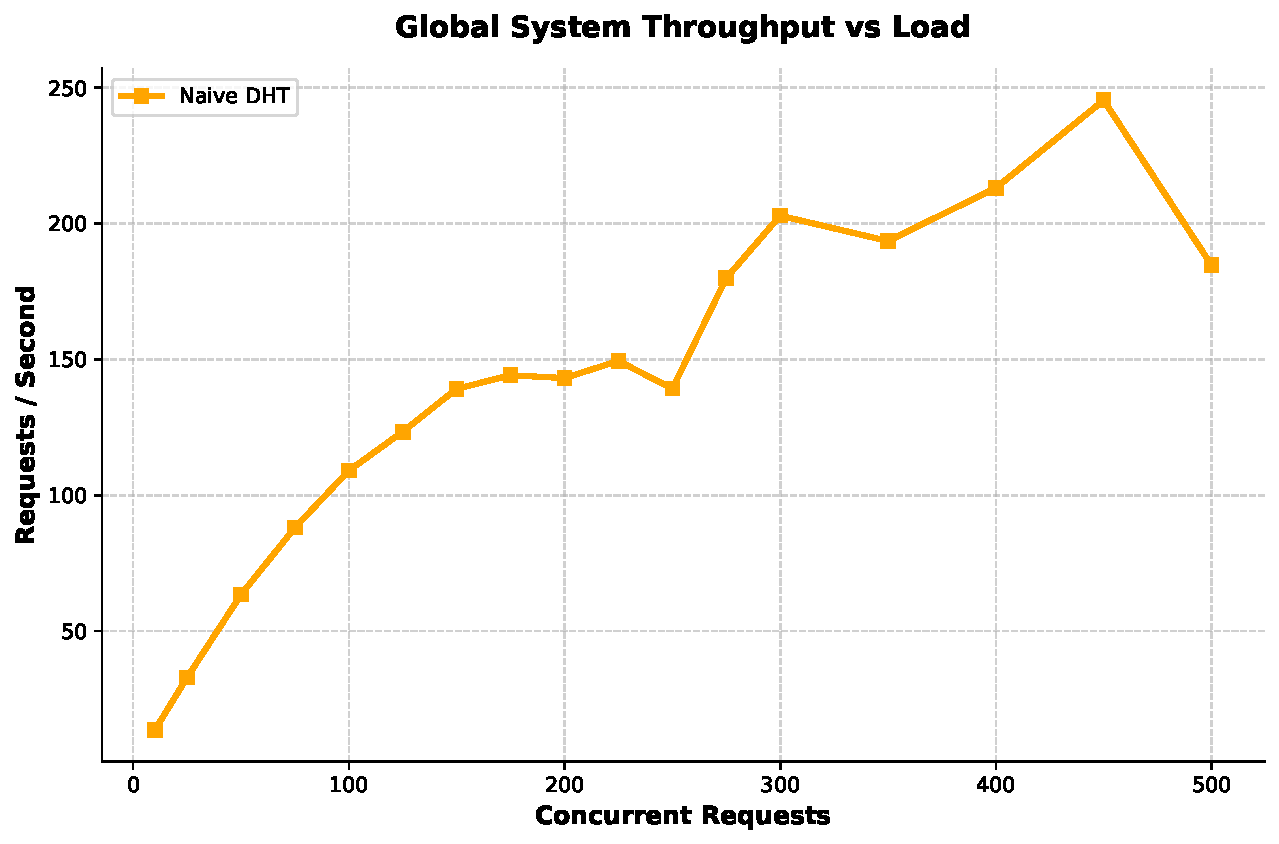
\includegraphics[width=0.40\textwidth]{graphs/pdf/dht_throughput.pdf}
    \caption{Débit global du système en fonction de la charge dans la DHT naïve.}
    \label{fig:naive_metrics_throughput}
\end{wrapfigure}

La Figure~\ref{fig:naive_metrics_throughput} montre une croissance initiale marquée du débit, suivie d'un plateau asymptotique. Dans la première phase, le système absorbe efficacement l'augmentation du nombre de requêtes concurrentes : tant que les ressources de calcul, les sockets et les threads disponibles ne sont pas saturés, une augmentation de la charge se traduit naturellement par une augmentation du débit total.

Cette lecture est cohérente avec la loi de Little,
\[
L = \lambda \cdot W,
\]
où \(L\) désigne le nombre moyen de requêtes présentes dans le système, \(\lambda\) le débit, et \(W\) le temps moyen de réponse. Tant que \(W\) reste modéré et que les ressources parallèles restent disponibles, \(\lambda\) peut continuer à croître avec la charge imposée. Le plateau observé indique en revanche l'apparition d'un goulot d'étranglement architectural. Dans une implémentation reposant sur des connexions TCP multiples et un modèle de traitement concurrent, ce plafonnement peut être lié à la saturation du nombre de threads utiles, à l'épuisement des ports éphémères, ou plus généralement à la capacité maximale de traitement parallèle de la JVM et du système hôte.

Une borne théorique simple du débit maximal peut alors s'écrire sous la forme
\[
\lambda_{max} \approx \frac{N_{threads}}{T_{process}},
\]
où \(N_{threads}\) désigne le nombre de traitements effectivement parallélisables et \(T_{process}\) le temps moyen nécessaire pour traiter une requête. Au-delà de ce seuil, l'ajout de nouvelles requêtes n'augmente plus réellement le débit ; il allonge surtout les files d'attente et accroît les surcoûts liés à l'ordonnancement, aux changements de contexte et à la contention. Le plateau observé constitue donc un indicateur direct de la capacité limite de cette architecture non structurée dans le cadre expérimental retenu.

\newpage
\subsubsection{Efficacité du réseau : nombre moyen de sauts par requête}

\begin{wrapfigure}{r}{0.44\textwidth}
    \centering
    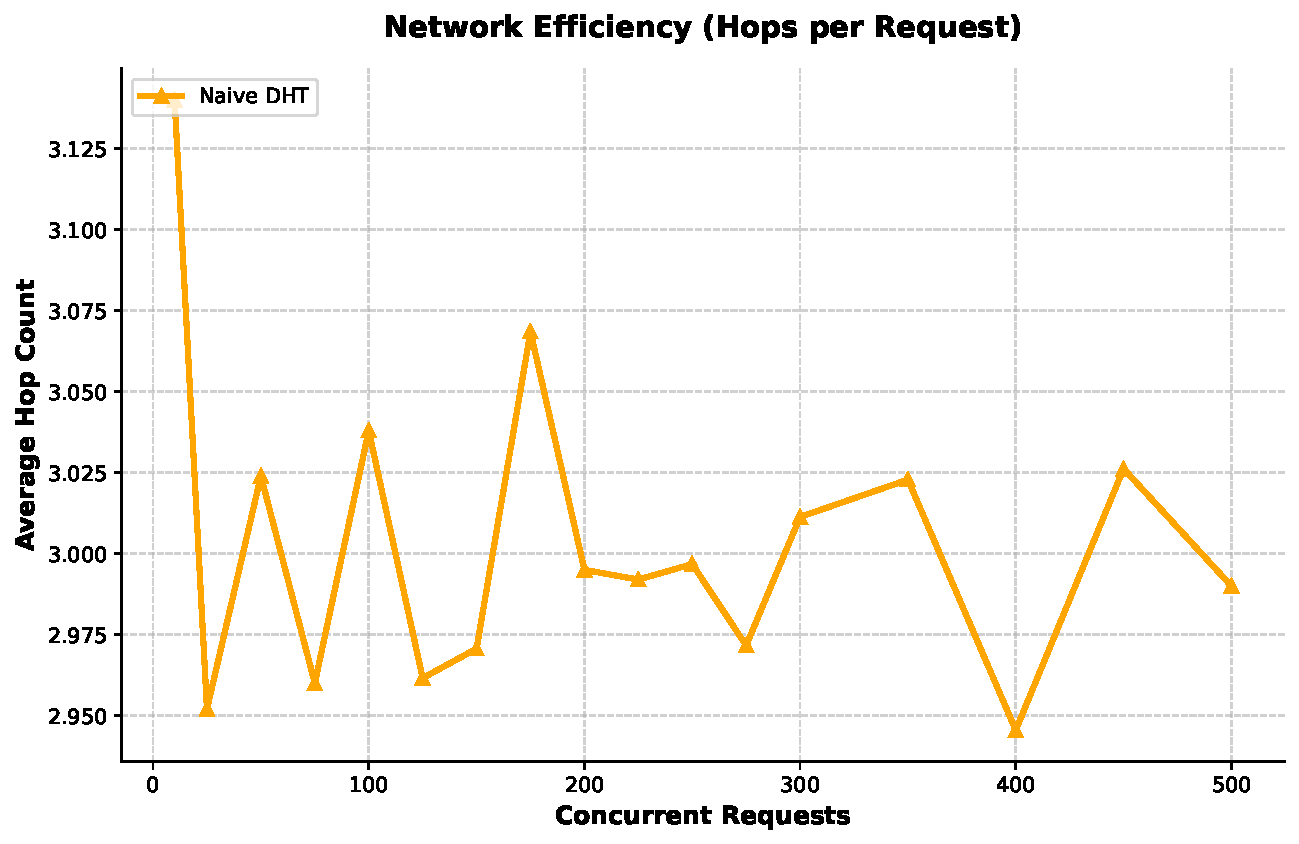
\includegraphics[width=0.40\textwidth]{graphs/pdf/dht_hops.pdf}
    \caption{Nombre moyen de sauts par requête dans la DHT naïve.}
    \label{fig:naive_metrics_hops}
\end{wrapfigure}

La Figure~\ref{fig:naive_metrics_hops} présente une courbe presque plate, oscillant faiblement autour d'une valeur voisine de trois sauts. Cette stabilité est un résultat important. Dans une architecture non structurée fondée sur l'inondation, le nombre de messages potentiellement engendrés par une requête peut croître très vite si rien ne vient limiter la propagation. Si \(k\) désigne le degré moyen des n\oe uds et \(t\) la profondeur maximale autorisée par le \textit{TTL}, le nombre total de messages générés peut être majoré par la série
\[
M = \sum_{i=1}^{t} k^i = \frac{k(k^t-1)}{k-1}.
\]
Sans filtrage efficace, un tel comportement conduirait rapidement à des tempêtes de diffusion.

Le fait que le nombre moyen de sauts reste pratiquement constant signifie précisément que ce pire cas n'est pas atteint en pratique dans les expériences réalisées. Deux facteurs l'expliquent. D'une part, le mécanisme d'élimination des doublons et l'enregistrement des routes empêchent les boucles et limitent fortement les retransmissions inutiles. D'autre part, la convergence vers un réseau très dense, favorisée par le \textit{pong caching}, réduit la distance géodésique effective entre les pairs. Dans un cluster local fortement connecté, cette distance reste presque constante quand la charge augmente. Le coût en sauts n'est donc pas déterminé par le nombre de clients simultanés, mais surtout par la structure topologique déjà atteinte par le réseau. Cette stabilité expérimentale est donc cohérente avec une topologie devenue quasi complète à petite échelle.

\subsubsection{Temps de convergence de la topologie}

\begin{wrapfigure}{l}{0.44\textwidth}
    \centering
    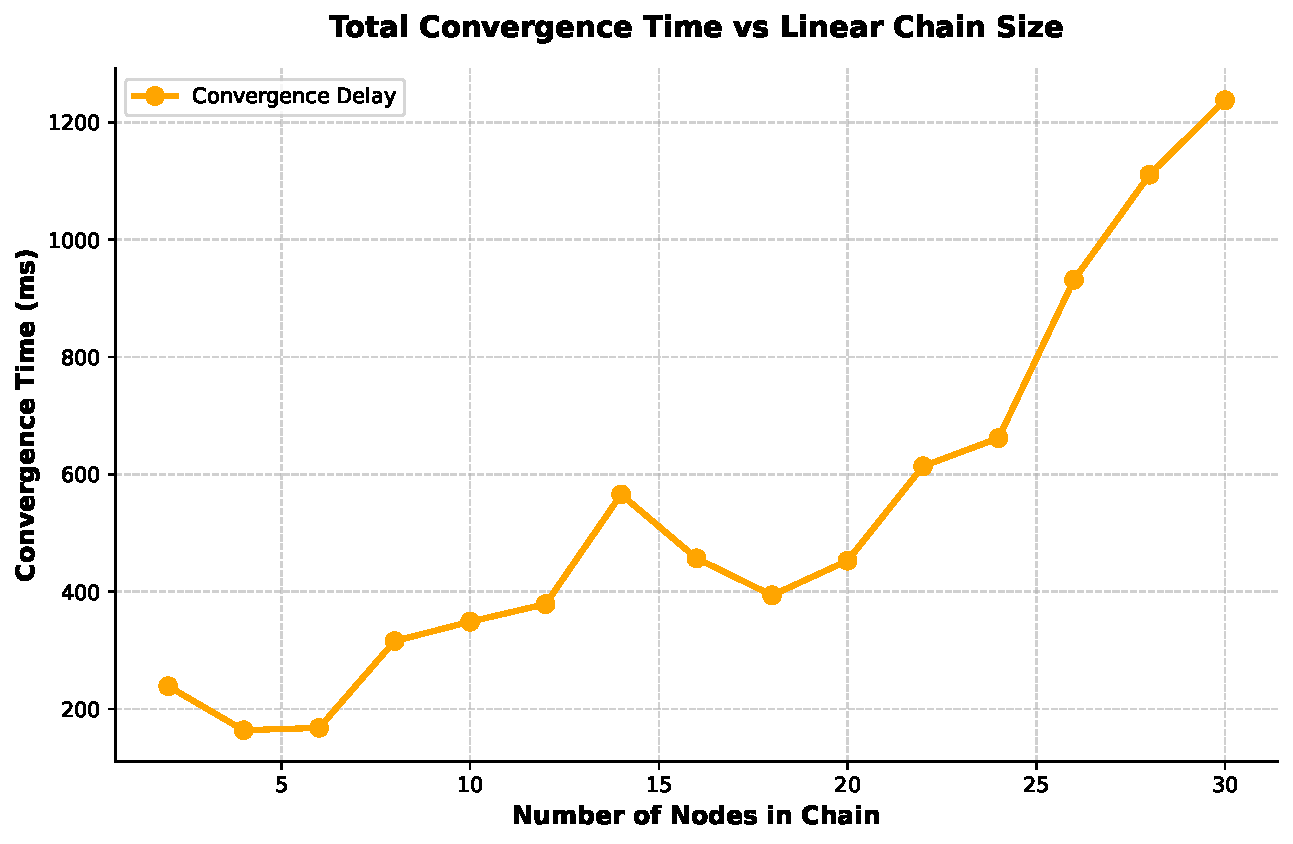
\includegraphics[width=0.40\textwidth]{graphs/pdf/dht_chain_convergence.pdf}
    \caption{Temps de convergence de la topologie dans une chaîne linéaire de n\oe uds.}
    \label{fig:naive_metrics_convergence}
\end{wrapfigure}

La Figure~\ref{fig:naive_metrics_convergence} a été mesurée dans un scénario volontairement défavorable : une chaîne linéaire de \(N\) n\oe uds, dans laquelle chaque pair ne connaît initialement que son voisin immédiat. La courbe obtenue est quasi linéaire, ce qui traduit une croissance proportionnelle du temps de convergence avec la taille du réseau.

Ce résultat est théoriquement attendu. Une architecture non structurée ne converge pas spontanément vers un maillage complet ; elle repose au contraire sur des échanges locaux d'information, ici via les messages \texttt{PING}/\texttt{PONG} enrichis par le \textit{pong caching}. Dans une chaîne, l'information concernant un n\oe ud situé à une extrémité du réseau doit être relayée séquentiellement de proche en proche jusqu'à l'autre extrémité. Si \(T_{hop}\) désigne le délai moyen de traitement et de transmission entre deux n\oe uds voisins, le temps total de convergence peut alors être approché par
\[
T_{conv} = (N-1) \cdot T_{hop},
\]
ce qui conduit directement à une complexité linéaire :
\[
T_{conv} \in O(N).
\]
Cette mesure confirme donc une limite structurelle importante de la DHT naïve. Même si le \textit{pong caching} améliore fortement la diffusion des adresses et permet, à petite échelle, une convergence rapide vers un mesh dense, le coût de propagation de l'état reste fondamentalement linéaire dans les scénarios défavorables. Cette propriété distingue nettement cette architecture des DHT structurées, dans lesquelles la découverte et le routage s'appuient sur des invariants topologiques plus forts et sur des garanties asymptotiques en \(O(\log N)\).

\subsubsection{Synthèse}

Pris ensemble, ces quatre graphes montrent que la DHT naïve ne doit pas être analysée comme un simple réseau d'inondation brut. Les mécanismes ajoutés au cours de son évolution --- en particulier le \textit{pong caching} pour la convergence topologique et le \textit{reverse path caching} pour la mise en cache opportuniste --- modifient profondément son comportement observé. La latence diminue lorsque le cache devient efficace, le débit croît jusqu'à une saturation imposée par les ressources d'exécution, le nombre moyen de sauts reste presque constant dans un cluster dense, et le temps de convergence révèle en même temps la limite fondamentale de passage à l'échelle d'une architecture non structurée. Cette lecture métrique éclaire donc directement la transition vers la génération suivante : malgré les gains obtenus, la nécessité d'un routage déterministe et d'une meilleure scalabilité motive naturellement l'adoption d'une DHT structurée.